\begin{figure}
\centering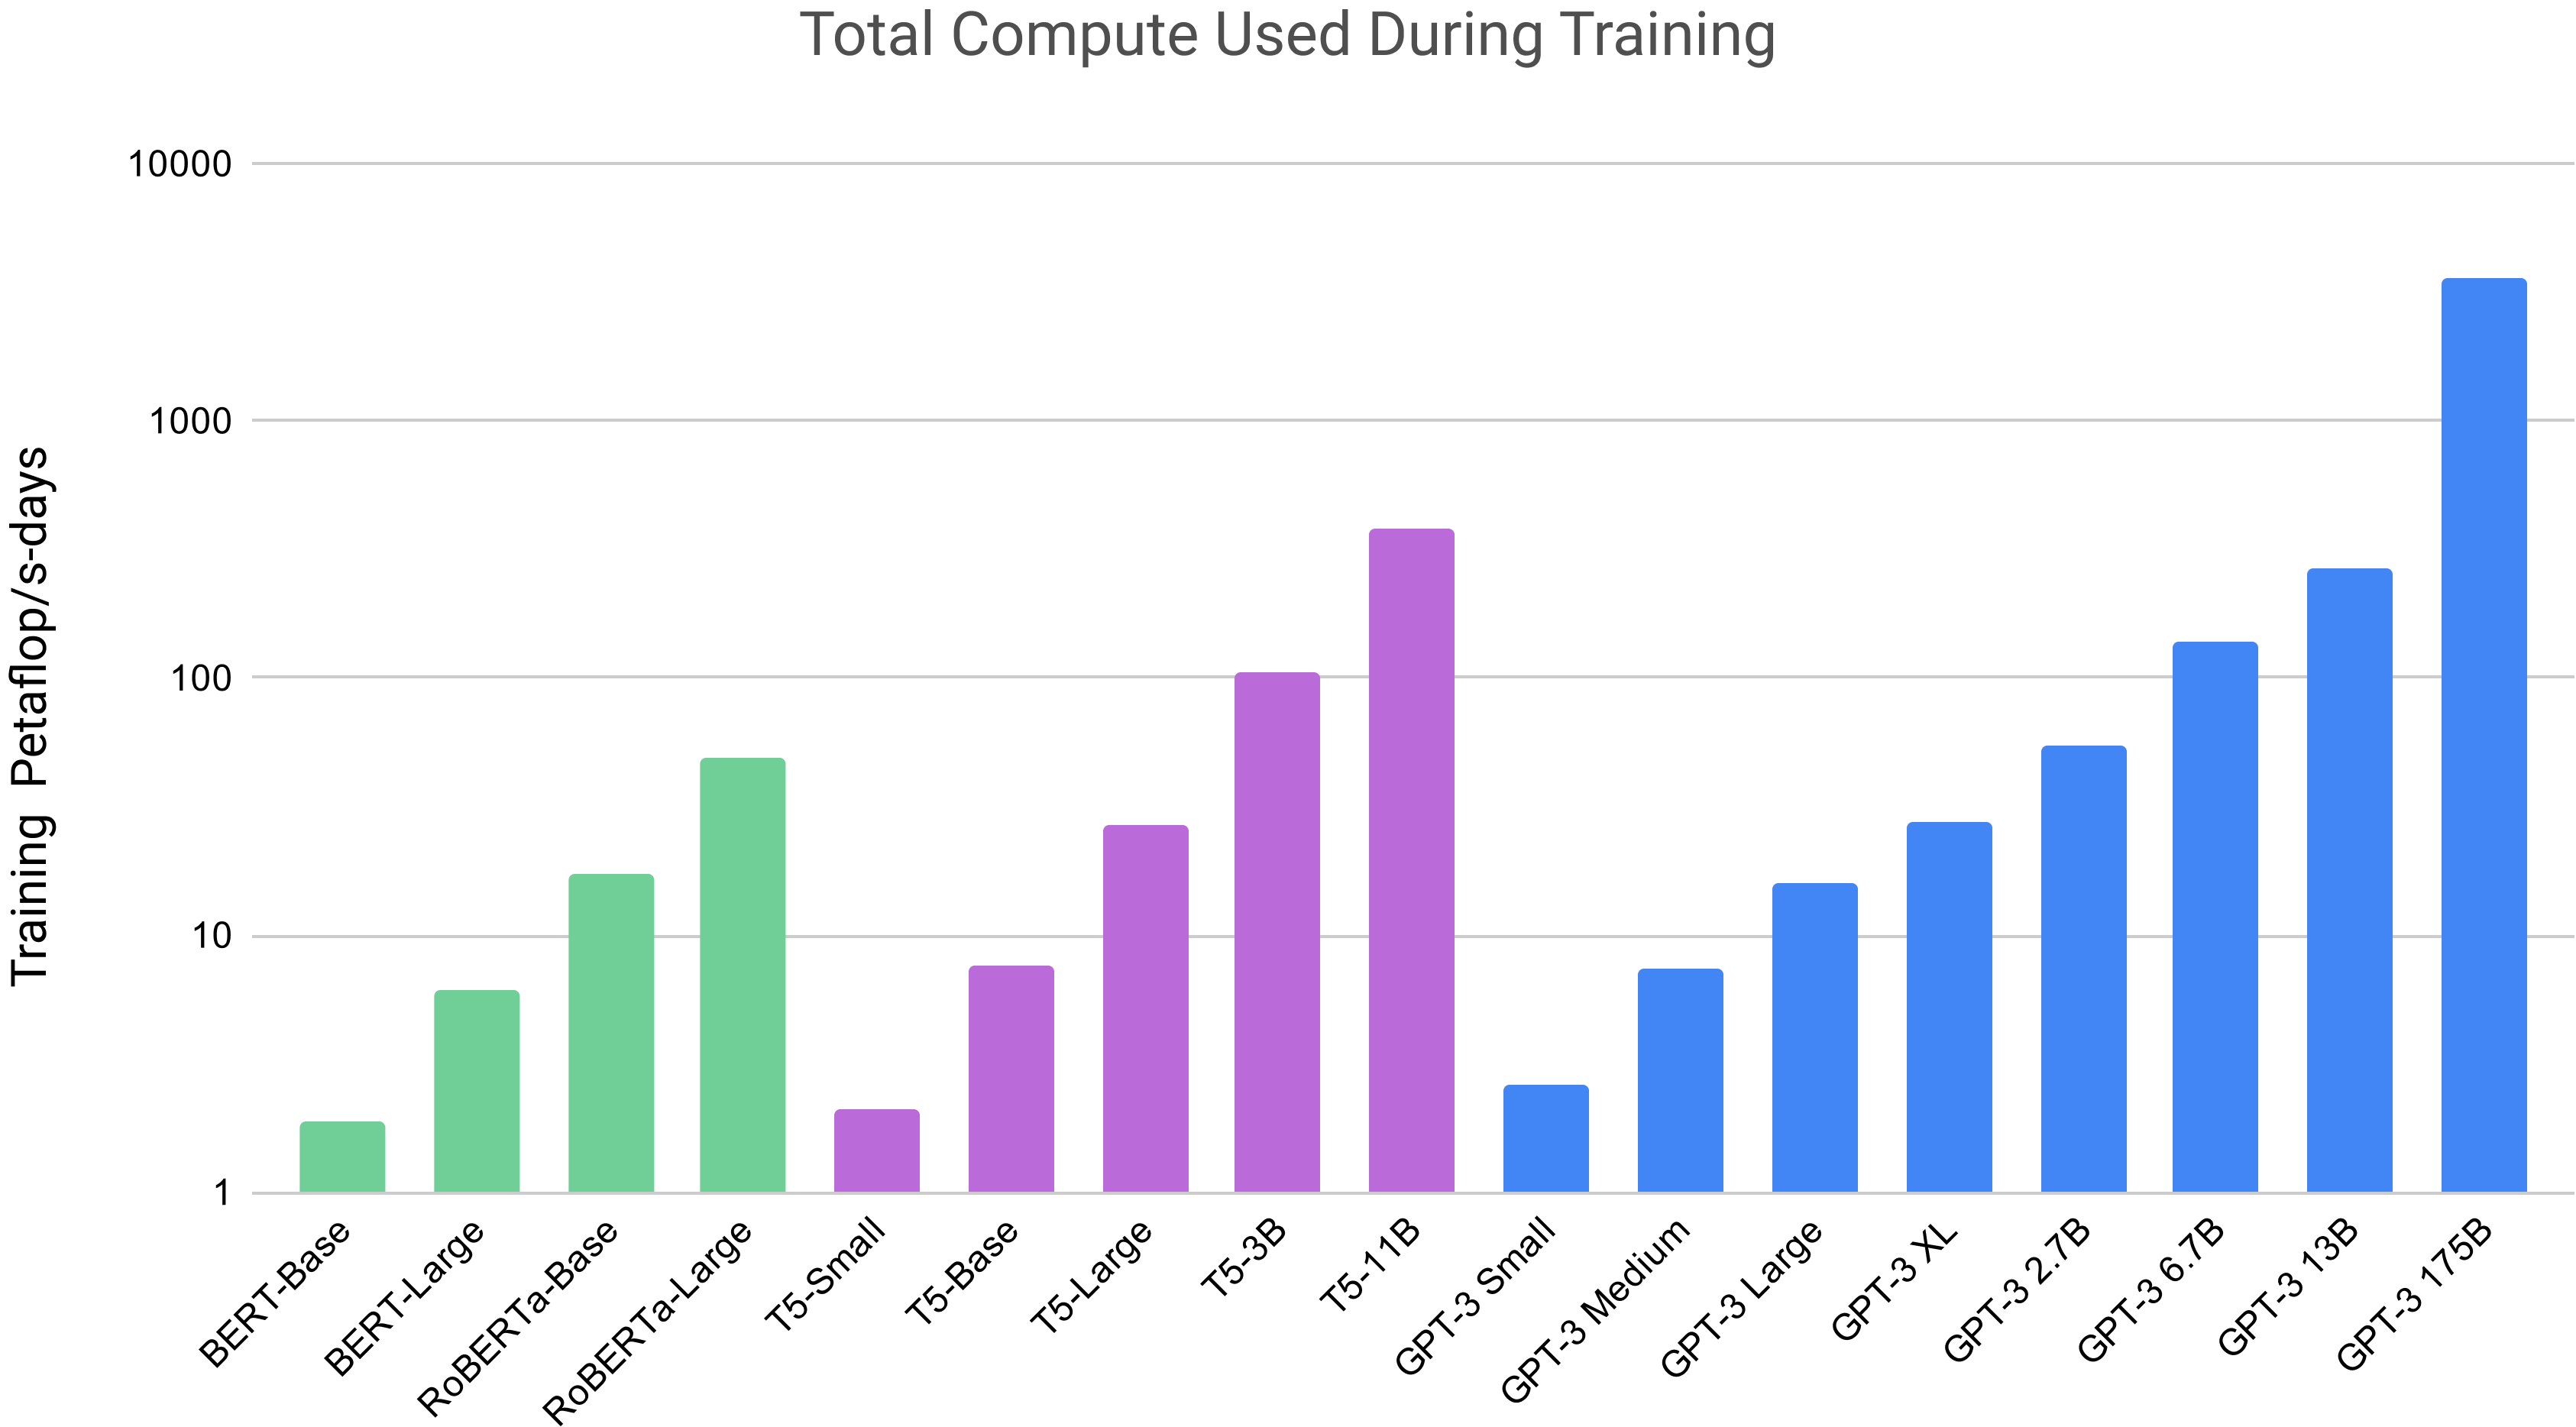
\includegraphics[width=0.9\linewidth]{figures/training_flops.png}
\caption{\textbf{Total compute used during training}. Based on the analysis in Scaling Laws For Neural Language Models \cite{kaplan2020scaling} we train much larger models on many fewer tokens than is typical. As a consequence, although GPT-3 3B is almost 10x larger than RoBERTa-Large (355M params), both models took roughly 50 petaflop/s-days of compute during pre-training. Methodology for these calculations can be found in Appendix \ref{appendix:total_compute_calculations}.
}
\label{figure:training flops}
\end{figure}
